% !TEX root = /Users/nai1ka/Projects/thesis_template/thesis.tex
\chapter{Implementation}
\label{chap:impl}

This chapter presents the implementation of the design introduced in Chapter~\ref{chap:met}. Section~\ref{sec:sdk_impl} covers the mobile SDK, from initialization to the individual collectors and the buffering and transmission pipeline. Section~\ref{sec:backend_impl} describes the backend server, focusing on user management and the ingestion path. Section~\ref{sec:frontend_impl} walks through the frontend web application and its main features. Section~\ref{sec:regression_impl} then explains the regression detection pipeline in detail.

\section{Mobile SDK Implementation}
\label{sec:sdk_impl}

The mobile part of the monitoring system was implemented as an Android library written in Kotlin. Kotlin was chosen because it is the official, recommended language for Android development~\cite{KotlinFirst}.


The SDK is distributed through a Maven repository, which allows developers to add it to their project easily by adding s dependency to their \texttt{build.gradle} file.

\subsection{Initialization and Lifecycle Management}

One of the requirements for the SDK was to make the integration as simple as possible for developers. To achieve this, the entire setup is done with a single call to the \texttt{PerfX.initialize()} method inside the application class. The developer only needs to provide the application context and a unique project ID.

Initialization runs a short sequence of steps. The \texttt{AppInfoProvider} collects device and app metadata (OS version, device model, app version). The SDK then opens the local Room database (\texttt{MetricDatabase}), starts the background sync manager, and creates the metric collectors. Finally, the SDK registers an \texttt{Application.ActivityLifecycleCallbacks} listener so it can follow the active screen and pause network sync while the app sits in the background, which saves battery.

\begin{lstlisting}[language=Kotlin, caption={SDK Initialization}]
fun initialize(application: Application, projectId: String) {
    if (isRunning) return

    appInfo = AppInfoProvider().get(application, projectId)
    db = MetricDatabase.getInstance(application)
    SyncManager.startPeriodicSync(application)

    // ... Collector initialization (described below)

    registerActivityCallback(application)
    isRunning = true
}
\end{lstlisting}

\subsection{Performance Metrics Collectors}

Each metric collector extends a common abstract class called \texttt{PerformanceCollector}. This class defines a single \texttt{collect()} method that returns a Kotlin \texttt{Flow} of \texttt{Metric} objects, which allows the SDK to treat all collectors in a uniform way.

\begin{lstlisting}[language=Kotlin, caption={PerformanceCollector Abstract Class}]
internal abstract class PerformanceCollector {
    abstract fun collect(intervalMs: Long): Flow<Metric>
    abstract fun stop()
}
\end{lstlisting}

All individual metric streams are merged into a single \texttt{Flow} inside the \texttt{MetricsRepository} class. This design makes it easy to add new collectors in the future without changing the rest of the pipeline.

\textbf{1. Memory Collector}

The \texttt{RamCollector} runs on a background thread and measures the memory footprint of the application at a fixed sampling interval. It uses two Android APIs: \texttt{Debug.getMemoryInfo()} to get the total PSS (Proportional Set Size) of the process, and the Java \texttt{Runtime} to calculate the current Java heap usage. The Java heap usage is calculated as the difference between the total allocated heap and the currently free heap. This value is what gets emitted as the metric, because it reflects the memory actually used by the application code.

\begin{lstlisting}[language=Kotlin, caption={Memory Collector Implementation}]
val memoryInfo = Debug.MemoryInfo()
Debug.getMemoryInfo(memoryInfo)

val runtime = Runtime.getRuntime()
val javaHeapUsedMb = (runtime.totalMemory() - runtime.freeMemory()) / (1024.0 * 1024.0)
val pssMb = memoryInfo.totalPss / 1024.0

emit(Metric.MemoryUsage(timestamp = System.currentTimeMillis(), value = javaHeapUsedMb))
\end{lstlisting}

\textbf{2. CPU Collector}

Because modern Android versions restrict direct access to the \texttt{/proc/stat} file for security reasons, the \texttt{CpuCollector} uses the \texttt{android.os.Process} API instead. It measures CPU usage by recording the elapsed CPU time of the application process at two moments in time, separated by the sampling interval. The CPU usage percentage is then calculated as the ratio of the CPU time consumed during the interval to the total wall-clock time of that interval:

\begin{equation}
CPU\% = \frac{\Delta CPU_{process}}{\Delta t_{wall}} \cdot 100
\end{equation}

This approach gives a normalized measure of how much CPU time the application actually consumed relative to real time, which makes the values comparable across devices with different numbers of cores.

\textbf{3. Frame Time Collector}

To measure frame rendering time, the SDK registers a \texttt{Choreographer.FrameCallback} on the main thread. Android calls this callback every time a new frame is about to be drawn, passing the frame timestamp in nanoseconds. The collector calculates the time difference between two consecutive callbacks to get the raw frame time. Individual frame times are accumulated over a fixed interval and then averaged before being emitted as a single metric. This aggregation reduces the number of data points that need to be stored and transmitted, while still capturing the overall rendering performance of the window.

\begin{lstlisting}[language=Kotlin, caption={Frame Time Collector — core measurement}]
val callback = Choreographer.FrameCallback { frameTimeNs ->
    if (lastFrameTimeNs != 0L) {
        val deltaMs = (frameTimeNs - lastFrameTimeNs) / 1_000_000.0
        if (deltaMs >= 0.0) {
            frameCount++
            totalFrameTimeMs += deltaMs
        }
    }
    lastFrameTimeNs = frameTimeNs
    Choreographer.getInstance().postFrameCallback(frameCallback)
}

// Emitted every intervalMs
val avgFrameTime = if (frameCount > 0) totalFrameTimeMs / frameCount else 0.0
emit(Metric.FrameTime(timestamp = System.currentTimeMillis(), value = avgFrameTime))
\end{lstlisting}

\textbf{4. Startup Time Collector}

Startup time is measured by recording the timestamp at the moment the application process starts and comparing it to the timestamp of the first fully drawn frame. The SDK uses the \texttt{reportFullyDrawn()} API to detect when the first screen has finished rendering. The difference between these two timestamps is reported as the startup time.

\textbf{5. Interaction Delay Collector}

User interaction delay is measured by intercepting touch events on the root view of each activity. When a touch event is received, its timestamp is recorded. The delay is then calculated as the time between the touch event and the first frame rendered after the event was processed, which is detected using the \texttt{Choreographer} callback.

\textbf{6. ANR Detector}

The SDK detects ANR events using a watchdog pattern. A background thread posts a short task to the main thread's \texttt{Handler} and waits for it. If the task does not run within the timeout (5 seconds by default, matching the official Android documentation~\cite{AndroidVitals}), the watchdog treats the main thread as blocked and records an ANR. The approach needs no special permissions and works on every Android version.

\begin{lstlisting}[language=Kotlin, caption={ANR Watchdog — detection logic}]
val mainHandler = Handler(Looper.getMainLooper())
var mainThreadResponded = false

mainHandler.post { mainThreadResponded = true }
Thread.sleep(ANR_TIMEOUT_MS)

if (!mainThreadResponded) {
    emit(Metric.Anr(timestamp = System.currentTimeMillis()))
}
\end{lstlisting}

\subsection{Data Buffering and Network Transmission}

The SDK uses a two-tier buffering approach to make sure that no metrics are lost if the application crashes or the network is temporarily unavailable.

\textbf{Tier 1: In-Memory Buffer}

As metrics arrive from the various collectors, they are first stored in a \texttt{ConcurrentLinkedQueue}. This data structure was chosen because multiple collectors produce data concurrently on different background threads, and using a standard list could cause race conditions. The \texttt{ConcurrentLinkedQueue} allows safe concurrent access without explicit locking, which keeps the overhead low.

When the number of items in the memory buffer reaches a predefined limit (\texttt{MEMORY\_LIMIT}), the buffer is flushed to disk.

\begin{lstlisting}[language=Kotlin, caption={In-Memory Buffering}]
flow.collect { metric ->
    memoryBuffer.add(metric)
    memoryBufferSize += 1

    if (memoryBufferSize >= Constants.MEMORY_LIMIT) {
        flushToDisk(db, context)
        memoryBufferSize = 0
    }
}
\end{lstlisting}

\textbf{Tier 2: Disk Storage and Network Synchronization}

When the memory buffer is flushed, the metrics are saved to a local SQLite database managed by the Room library. Each record is saved together with the name of the currently visible screen, which is tracked by the lifecycle callback registered during initialization.

When the number of records in the database reaches \texttt{DISK\_LIMIT}, an immediate network synchronization is triggered. In addition, a periodic background job runs every 15 minutes to synchronize any remaining records, even if the size threshold has not been reached. This ensures that metrics are uploaded even when the application is used infrequently.

The network layer is implemented using Retrofit and OkHttp. A batch of records is retrieved from the database, serialized into JSON using Kotlinx Serialization, and sent to the backend via a single HTTP POST request. If the request succeeds, the uploaded records are deleted from the local database. If it fails, the records remain on disk and are retried during the next synchronization.

\begin{lstlisting}[language=Kotlin, caption={Network Synchronization}]
val batchApi = BatchApi(
    appInfo = PerfX.appInfo,
    metrics = batch.map { it.mapToApi() }
)

val response = NetworkClient.api.uploadBatch(batchApi)

if (response.isSuccessful) {
    db.metricDao().deleteMetrics(batch.map { it.id })
}
\end{lstlisting}

\section{Backend Server Implementation}
\label{sec:backend_impl}

The backend server was built using Kotlin and the Ktor framework. Ktor is a lightweight, asynchronous framework that is well suited for building REST APIs. It handles each incoming request on a coroutine, which allows it to process many connections at the same time without blocking threads.

The backend uses two separate database systems: PostgreSQL for relational data such as user accounts and project settings, and ClickHouse for time-series performance metrics.

\subsection{User and Project Management}

User accounts, projects, and regression detection configurations are stored in PostgreSQL. Figure~\ref{fig:postgres_schema} shows the database schema.

\begin{figure}[htbp]
    \centering
    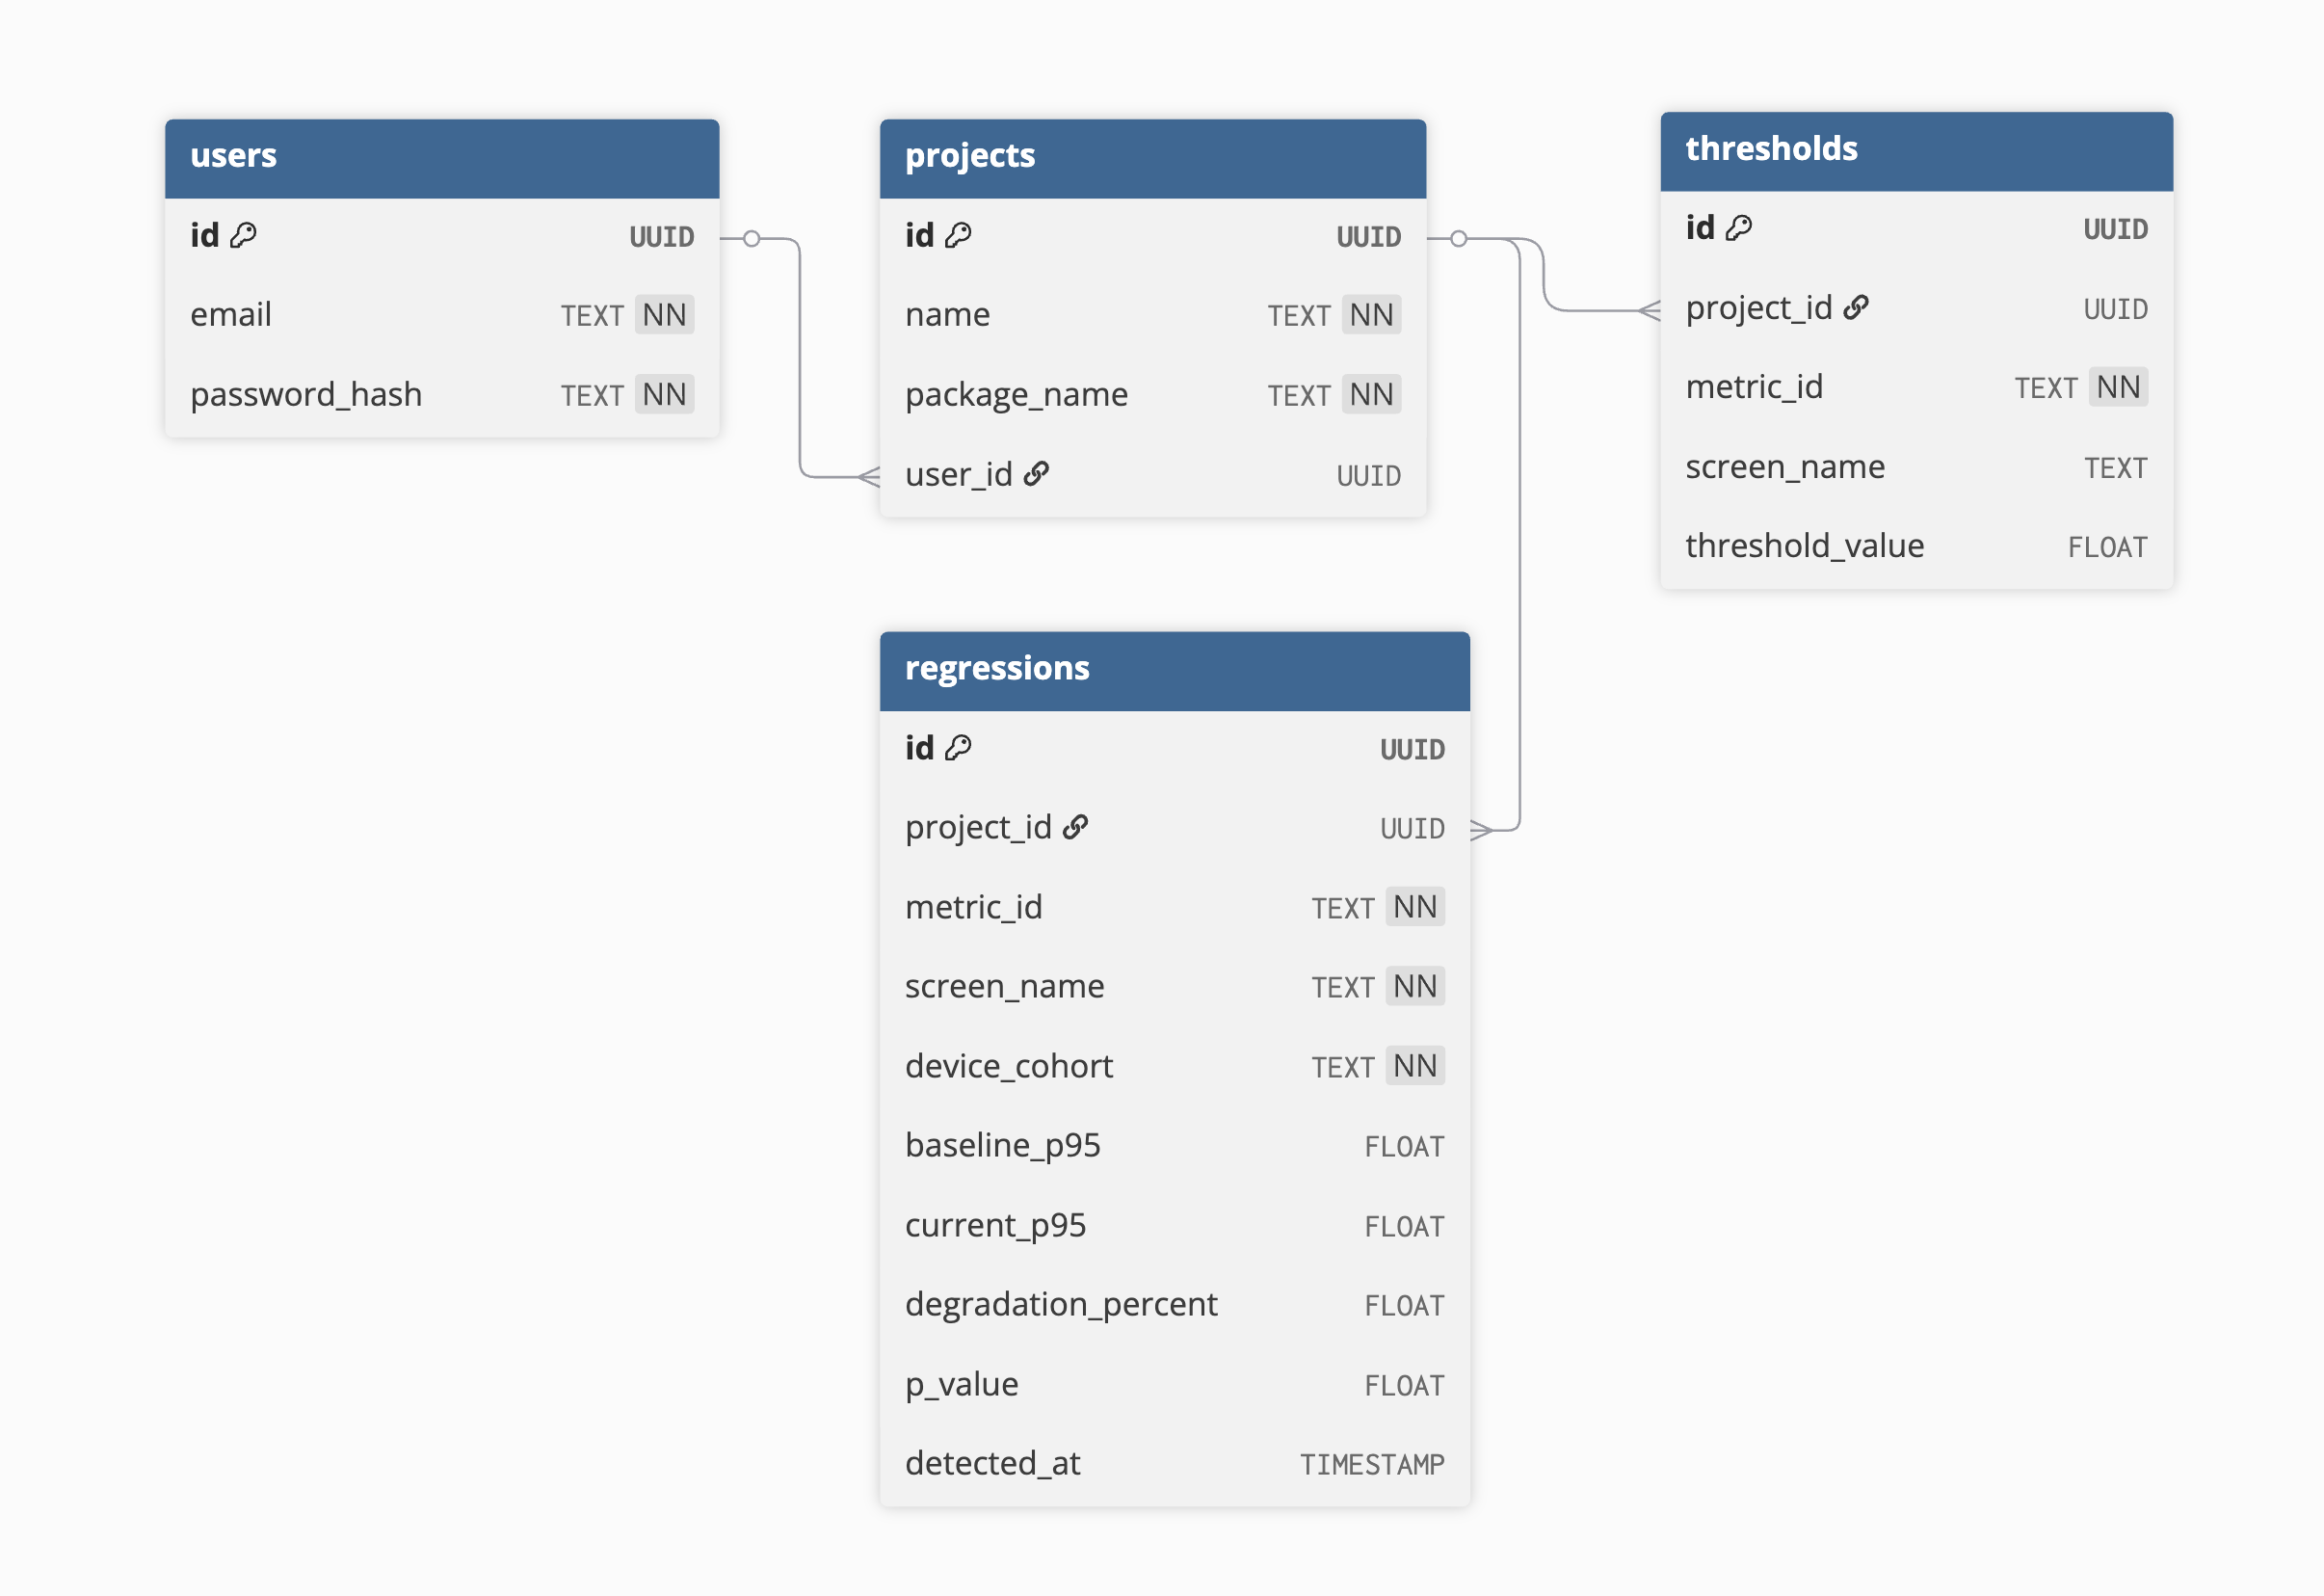
\includegraphics[width=0.8\textwidth]{figs/postgres_schema.png}
    \caption{PostgreSQL database schema}
    \label{fig:postgres_schema}
\end{figure}

User passwords are never stored in plain text. Before saving a password, the server hashes it using the BCrypt algorithm. When a user logs in, the server verifies the provided password against the stored hash. After a successful login, the server generates a JWT token using the \texttt{JwtConfig} object. This token must be included in all subsequent requests to the API, which ensures that users can only access data belonging to their own projects.

When a developer creates a new project, the server checks that the project name and Android package name are not already taken. If the validation passes, the project is saved and linked to the user's account. The \texttt{thresholds} table allows developers to define custom P95 degradation thresholds for specific metrics and screens. By default, the regression detection pipeline uses a global threshold of 15\% for all metrics. However, different metrics have different levels of natural variability. For example, frame time is relatively stable, so even a 10\% shift may indicate a real problem. CPU usage, on the other hand, fluctuates more under normal conditions, so a 15\% threshold may produce too many false alarms. The \texttt{thresholds} table solves this by storing per-project and per-metric overrides. When the detection pipeline evaluates a cohort, it looks up the threshold using the following priority order: first, an exact match for the project, metric, and screen name; then a project-wide rule for that metric with no specific screen; and finally the global default. This design lets each developer tune the sensitivity of the system without changing any code.

\subsection{Data Ingestion}
\label{sec:ingestion}

The data ingestion endpoint is the most performance-critical part of the backend, because the mobile SDKs from many users can send large numbers of metrics at the same time. Storing this data in PostgreSQL would not be efficient enough for this workload. For this reason, all performance metrics are stored in ClickHouse, which is a column-oriented database optimized for fast batch insertions and analytical range queries over time~\cite{schulze2024clickhouse}.

The \texttt{metric\_records} table was designed to support the queries needed by the regression detection pipeline efficiently. The table uses the \texttt{MergeTree} engine, which is ClickHouse's default storage engine optimized for fast insertions and range scans. The data is partitioned by date so that queries over a recent time window only scan the relevant partitions. The primary sort key is \texttt{(project\_id, metric\_id, ts)}, which makes range queries over time for a specific project and metric very fast.

\begin{lstlisting}[language=SQL, caption={ClickHouse metric\_records table schema}]
CREATE TABLE IF NOT EXISTS metrics.metric_records
(
    project_id    String,
    package_name  String,
    ts            DateTime64(3, 'UTC'),
    metric_id     LowCardinality(String),
    screen_name   LowCardinality(String),
    value         Float64,
    app_version   LowCardinality(String),
    os_version    LowCardinality(String),
    device_model  LowCardinality(String),
    device_cohort LowCardinality(String) DEFAULT 'Unknown',
    received_at   DateTime DEFAULT now()
)
ENGINE = MergeTree
PARTITION BY toDate(ts)
ORDER BY (project_id, metric_id, ts);
\end{lstlisting}

Columns such as \texttt{metric\_id}, \texttt{screen\_name}, and \texttt{device\_cohort} use the \texttt{LowCardinality} type, which compresses repeated string values efficiently and speeds up \texttt{GROUP BY} queries on these columns. Figure~\ref{fig:clickhouse_schema} shows the structure of the table.

% \begin{figure}[htbp]
%     \centering
%     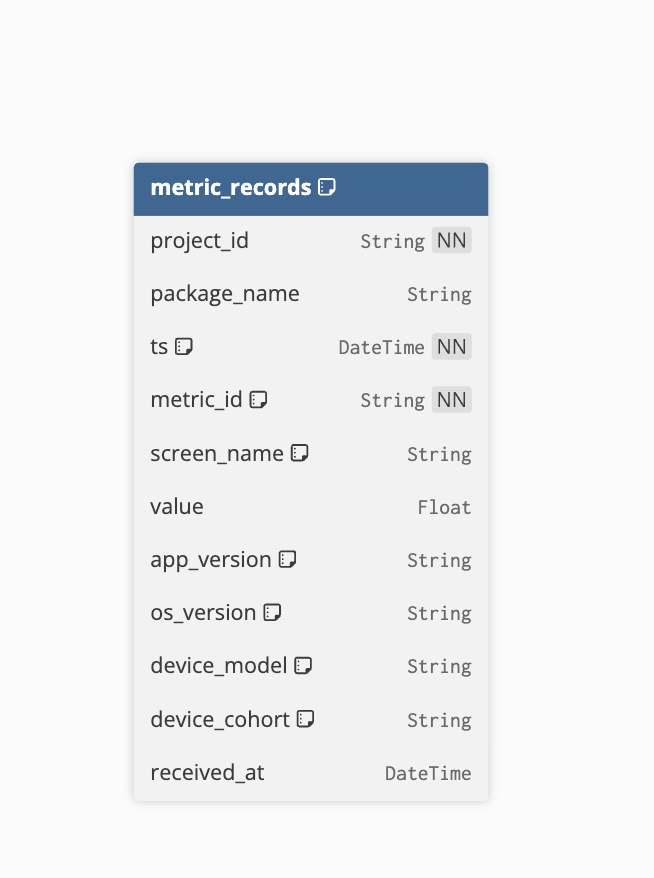
\includegraphics[width=0.7\textwidth]{figs/clickhouse_schema.png}
%     \caption{ClickHouse \texttt{metric\_records} table structure}
%     \label{fig:clickhouse_schema}
% \end{figure}

When the mobile SDK sends a POST request to the \texttt{/ingest} endpoint, the server receives a batch of metrics together with the application and device metadata. Instead of inserting each metric individually, the \texttt{ClickHouseClient} formats the entire batch as a single \texttt{JSONEachRow} payload and executes one bulk \texttt{INSERT} query. Before saving each record, the server also assigns the device cohort (Low, Medium, or High) based on the hardware metadata sent by the SDK. This batching approach keeps the load on the database low and allows the server to handle a large number of concurrent requests without becoming a bottleneck.

\section{Frontend Implementation}
\label{sec:frontend_impl}

The frontend was built using Streamlit, a Python framework for building interactive web applications. Streamlit was chosen because it allows data-driven dashboards to be created quickly, without the need for a separate frontend codebase. Charts and visualizations are rendered using Plotly.

\subsection{User Authorization}

Users can register and log in to the dashboard using their email and password. After a successful login, the JWT token received from the backend is stored in the browser session. All subsequent requests to the backend API include this token for authentication.

\begin{figure}[htbp]
    \centering
    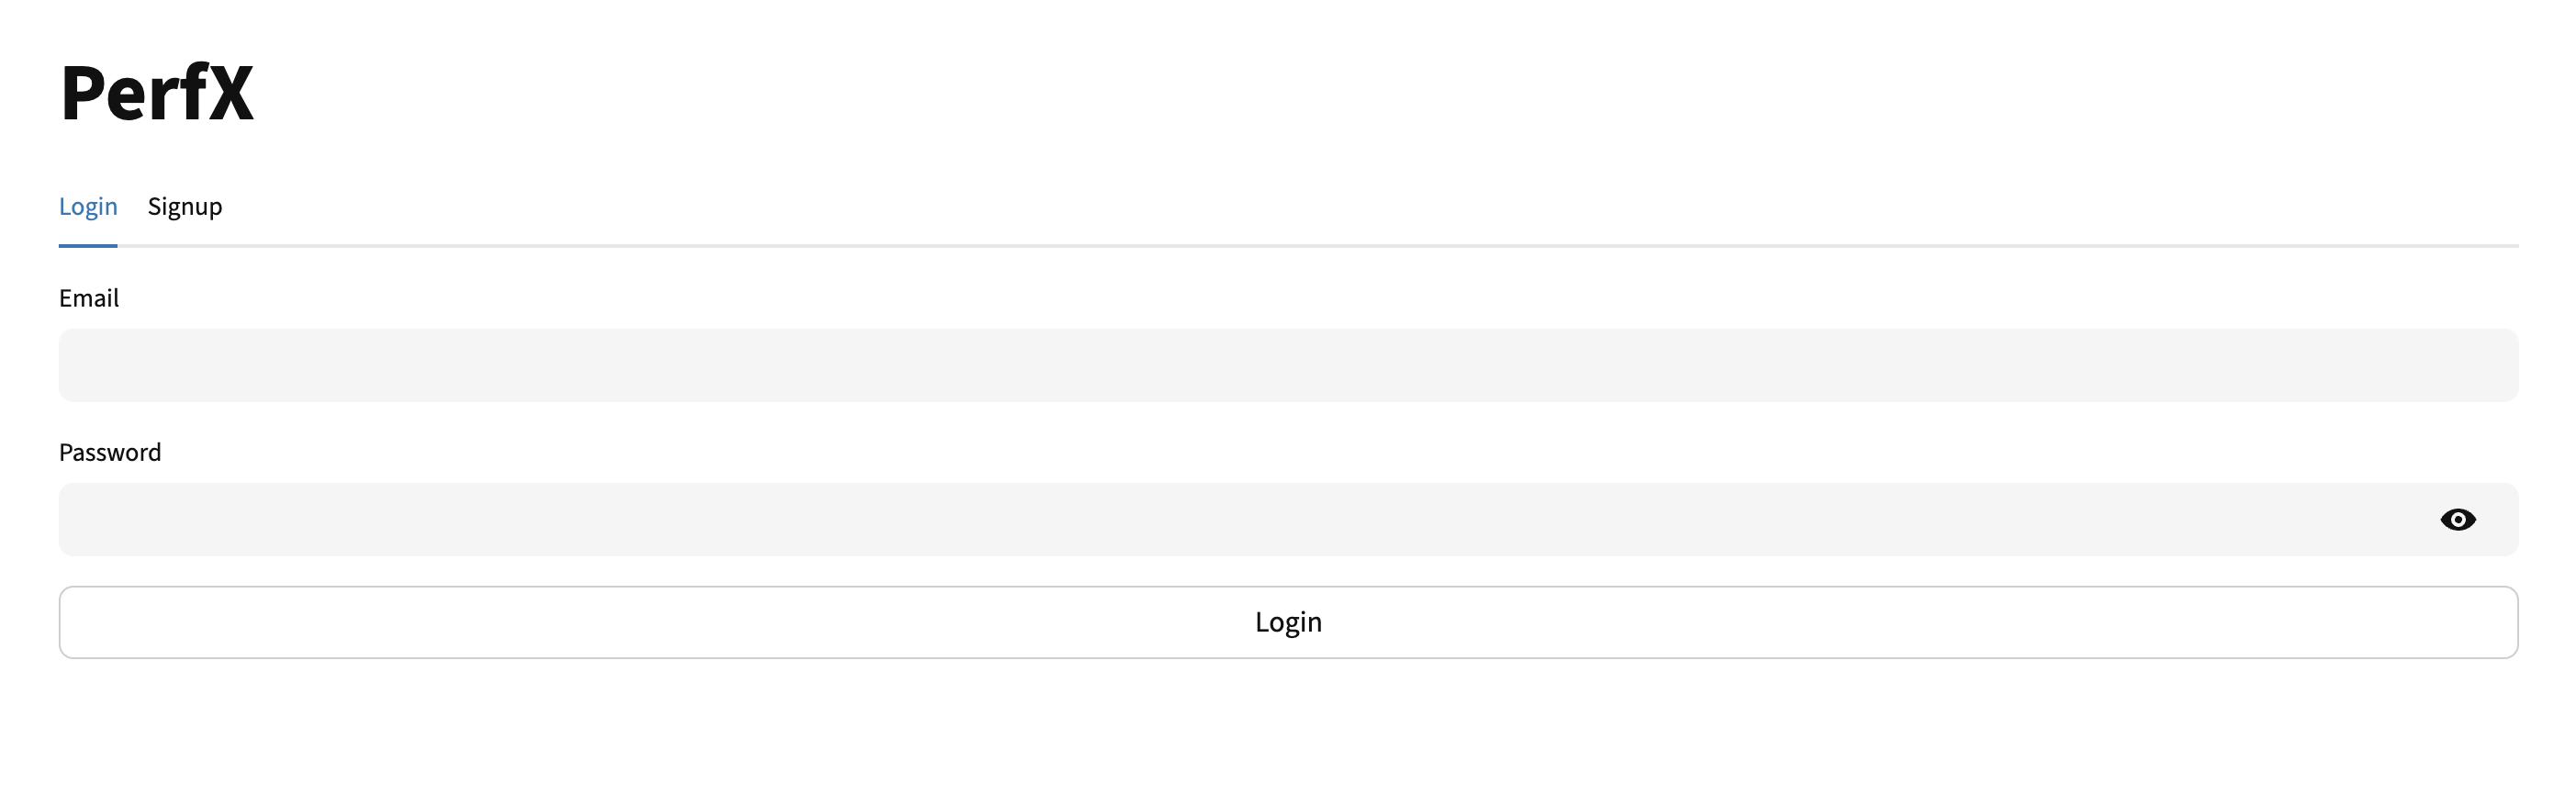
\includegraphics[width=0.8\textwidth]{figs/frontend_auth.png}
    \caption{Login page of the dashboard}
    \label{fig:auth_frontend}
\end{figure}

\subsection{Project Management}

After logging in, users can view a list of their existing projects, create new ones, and delete old ones. When a new project is created, the dashboard displays the unique project ID that the developer needs to use when initializing the mobile SDK in their Android application.

\begin{figure}[htbp]
    \centering
    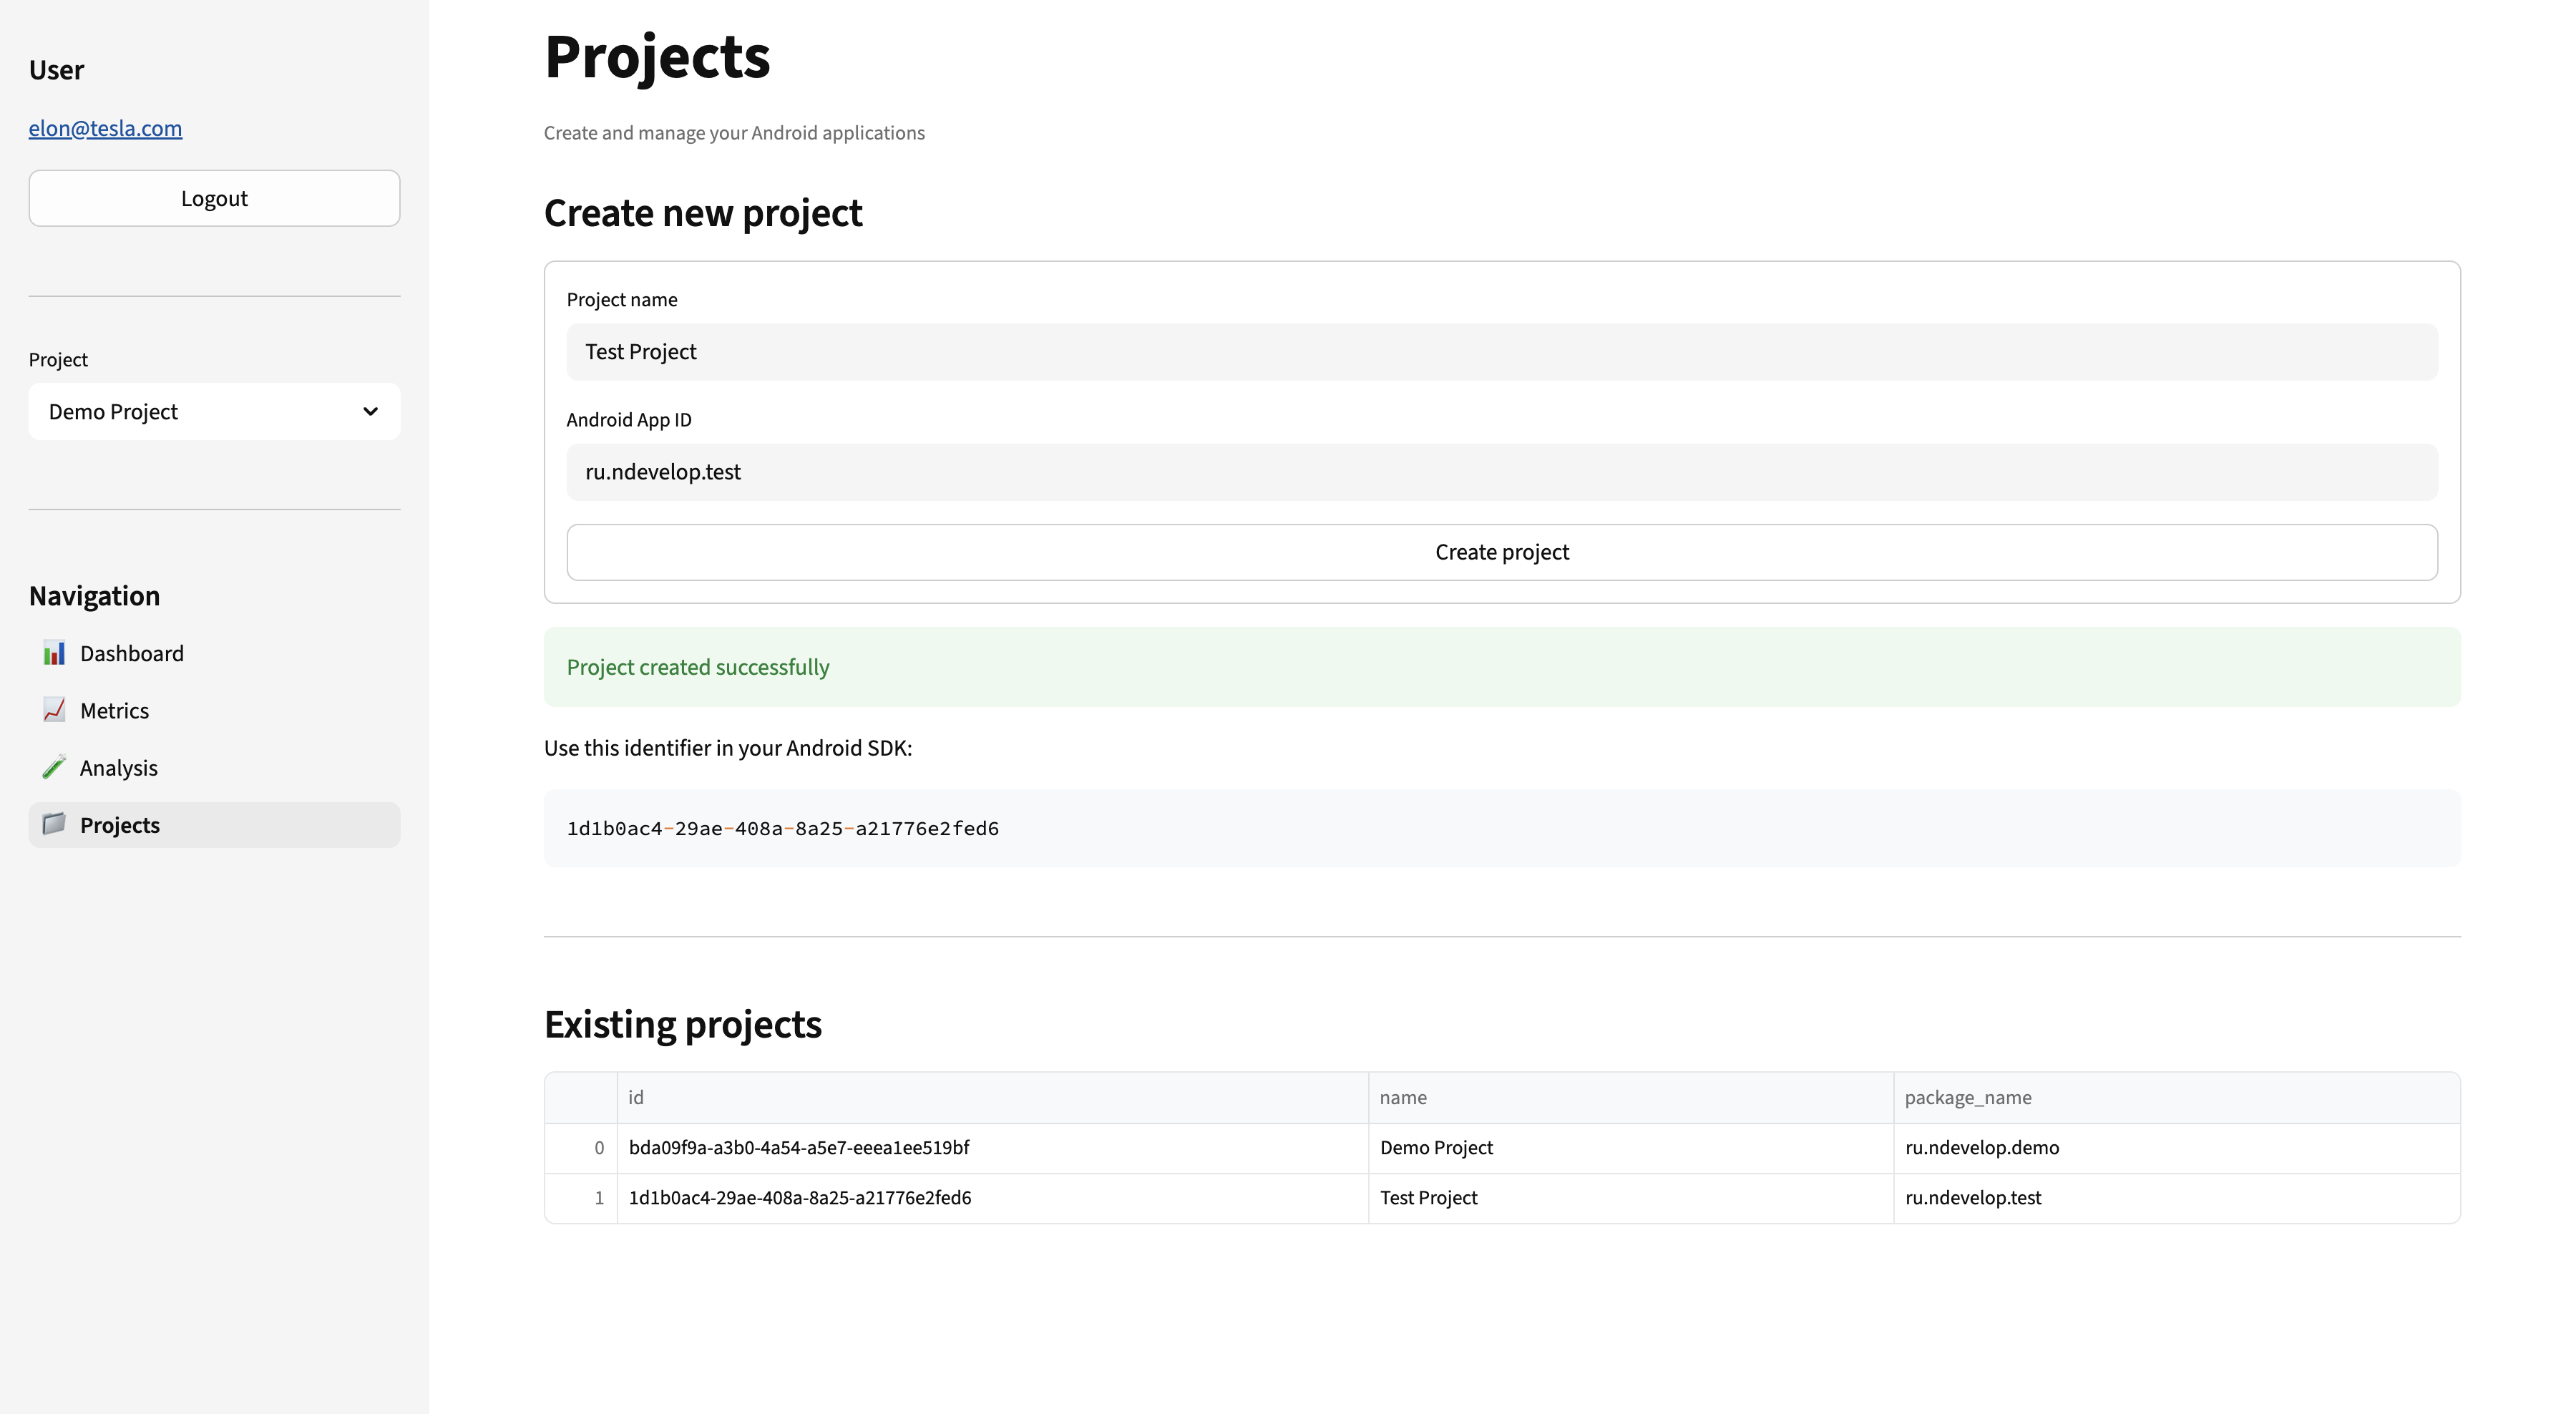
\includegraphics[width=0.8\textwidth]{figs/frontend_projects.png}
    \caption{Project list page}
    \label{fig:frontend_projects}
\end{figure}

\subsection{Dashboards}

The dashboard page allows users to visualize the collected metrics using interactive charts. Users can filter the data by time period, screen name, and device cohort to focus on a specific part of the application or a specific group of devices.

% \begin{figure}[htbp]
%     \centering
%     \includegraphics[width=0.8\textwidth]{figs/frontend_dashboard.png}
%     \caption{Dashboard page showing frame time metrics over time}
%     \label{fig:frontend_dashboard}
% \end{figure}

\subsection{Metrics Explorer}

The metrics explorer page shows the raw metric data in a table. Users can browse all collected measurements along with their timestamps, values, and associated metadata. The data can also be exported as a CSV file for further analysis in external tools such as Excel or Jupyter Notebook. This feature is useful for debugging or for performing custom analyses that go beyond what the standard dashboards offer.

\begin{figure}[htbp]
    \centering
    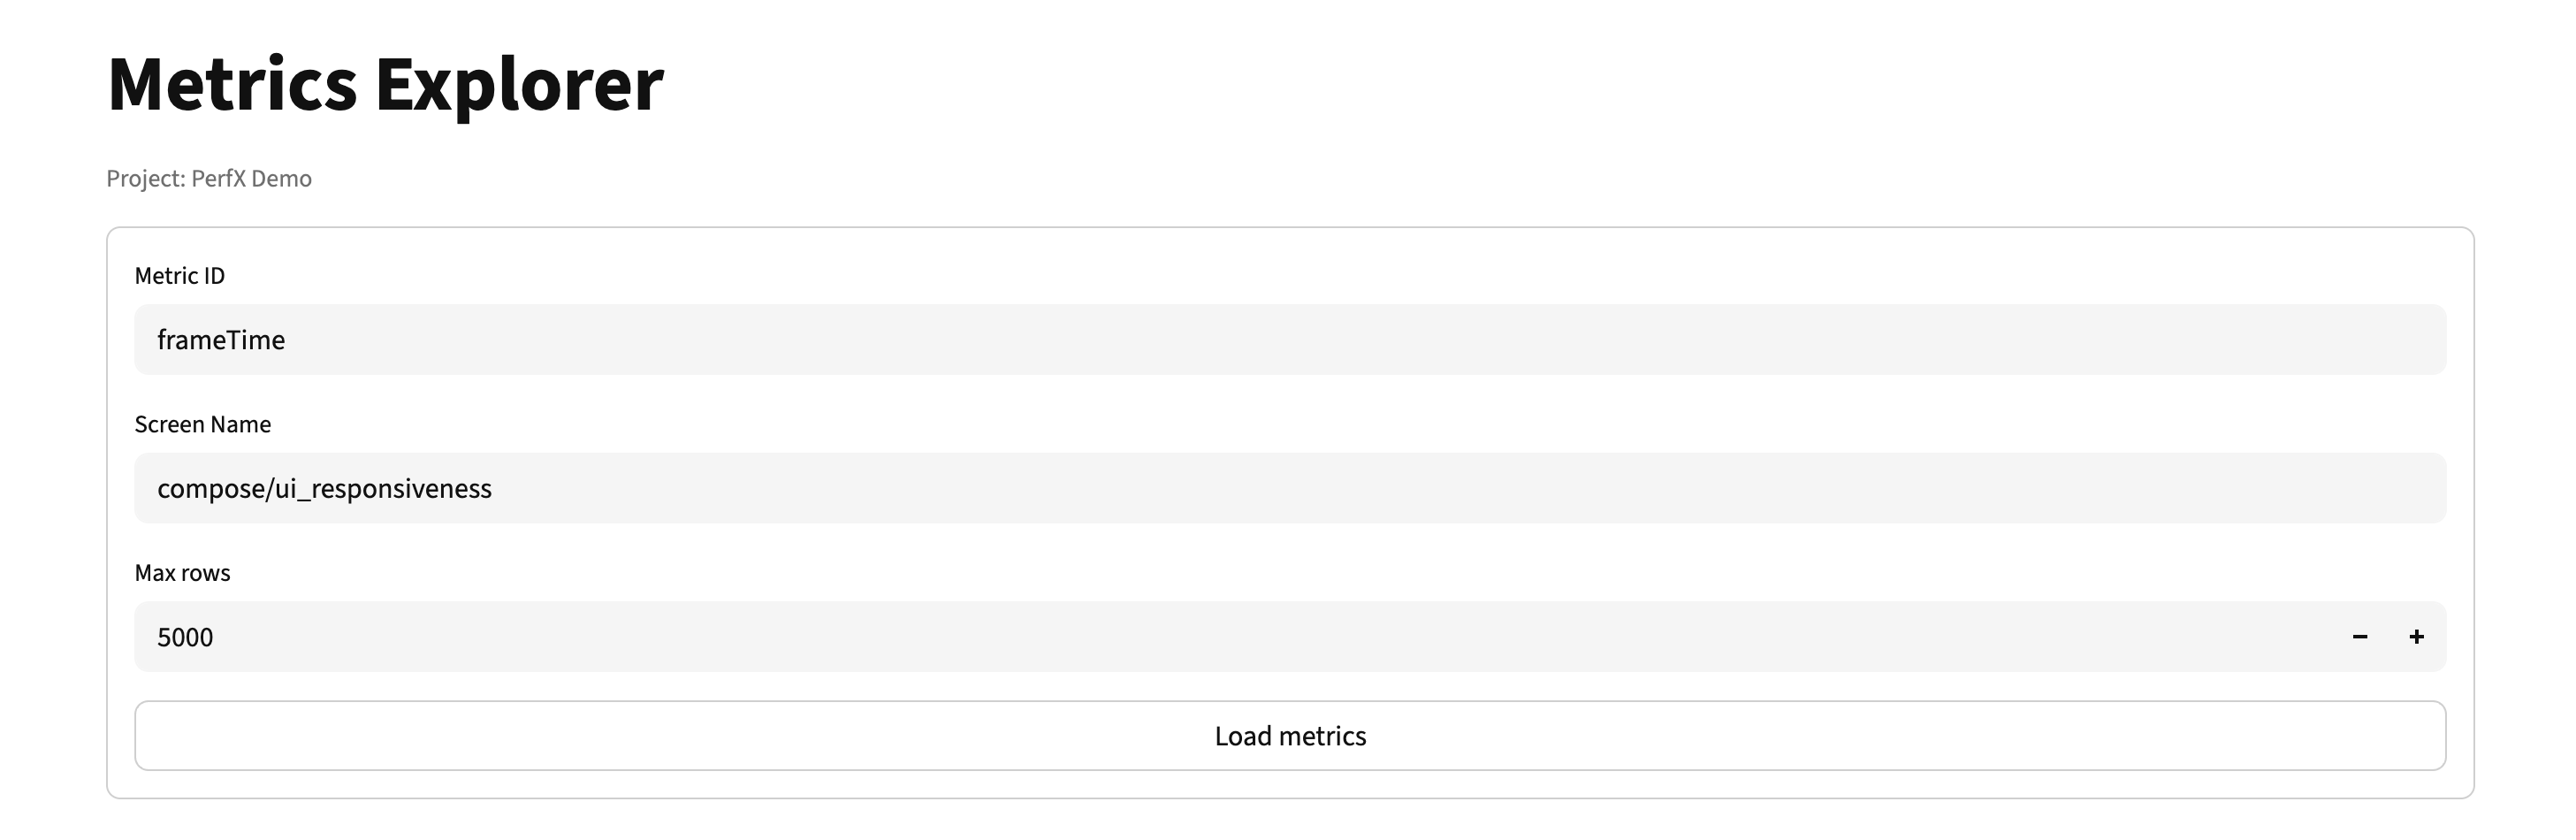
\includegraphics[width=0.8\textwidth]{figs/frontend_metrics_1.png}
    \caption{Metrics Explorer — filter selection}
    \label{fig:frontend_metrics_1}
\end{figure}

\begin{figure}[htbp]
    \centering
    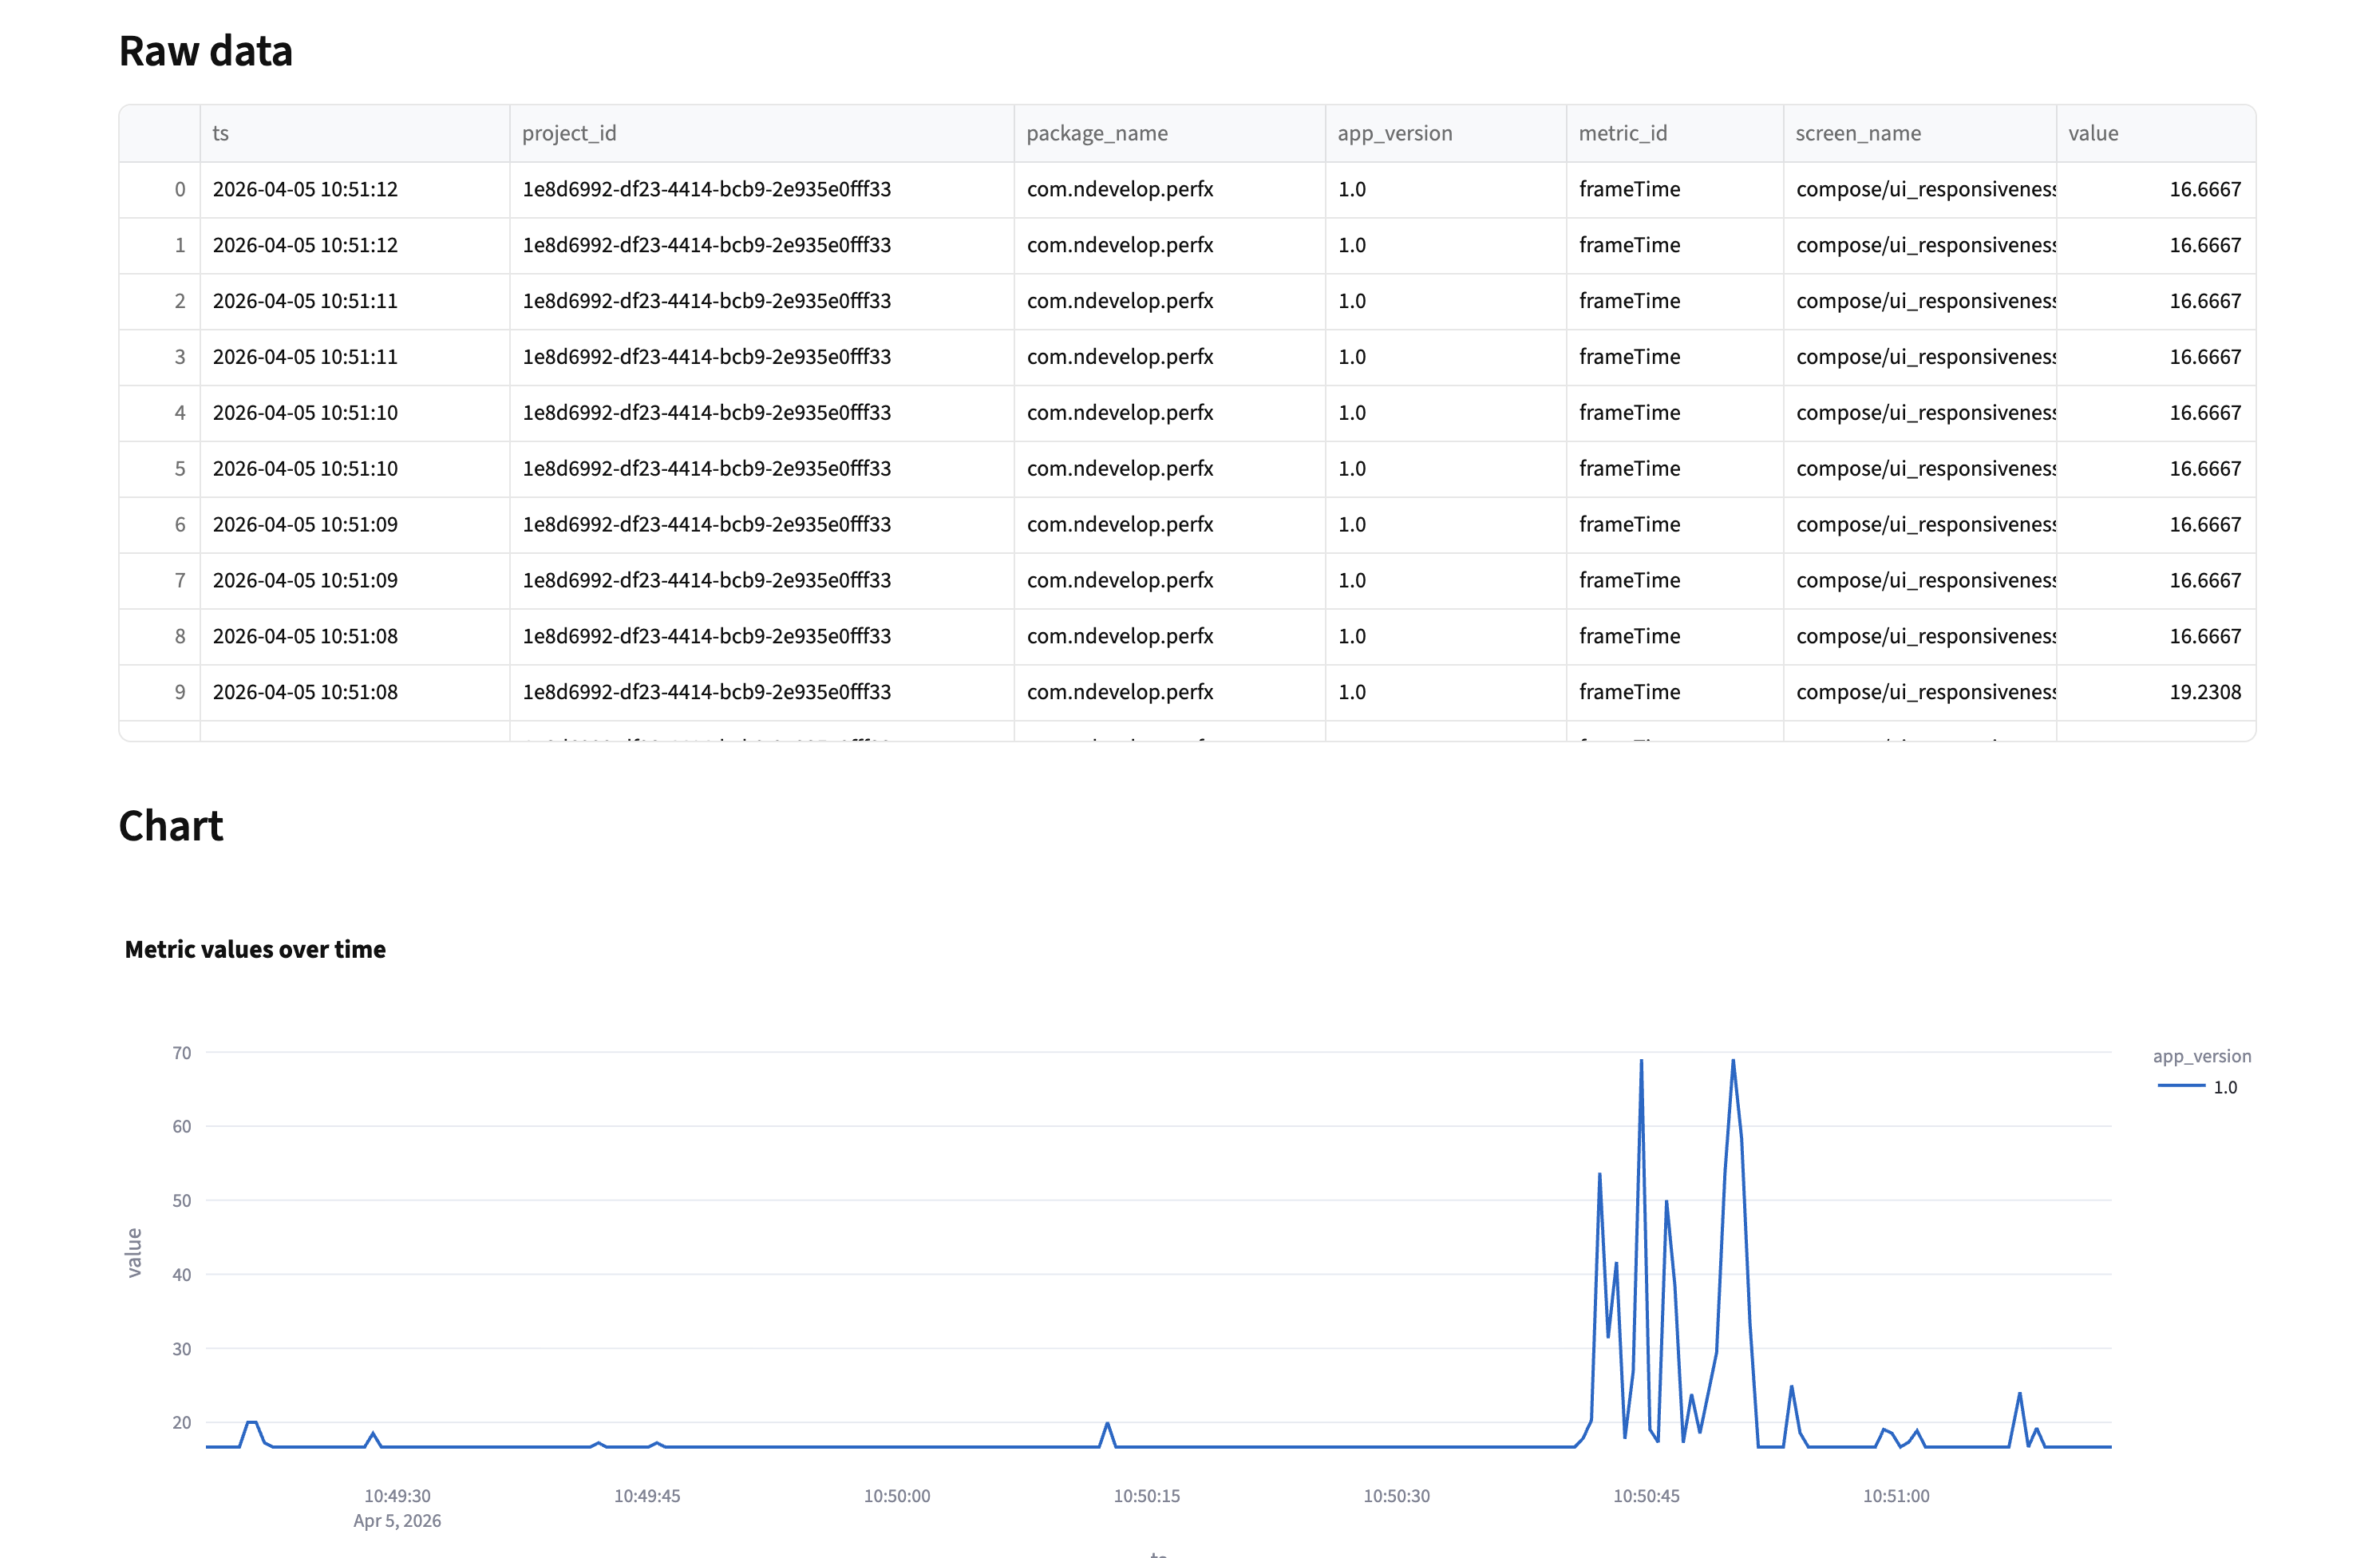
\includegraphics[width=0.8\textwidth]{figs/frontend_metrics_2.png}
    \caption{Metrics Explorer - frame time chart with a detected regression}
    \label{fig:frontend_metrics_2}
\end{figure}

\subsection{Alerting and Notifications}

The alerting page allows users to configure performance thresholds for specific metrics and screens. Users can also choose how they want to be notified when a regression is detected, for example by email or via a Telegram message. The sensitivity of the regression detection algorithm can be adjusted per metric and per screen by changing the relative degradation threshold stored in the \texttt{thresholds} table.
% \begin{figure}[htbp]
%     \centering
%     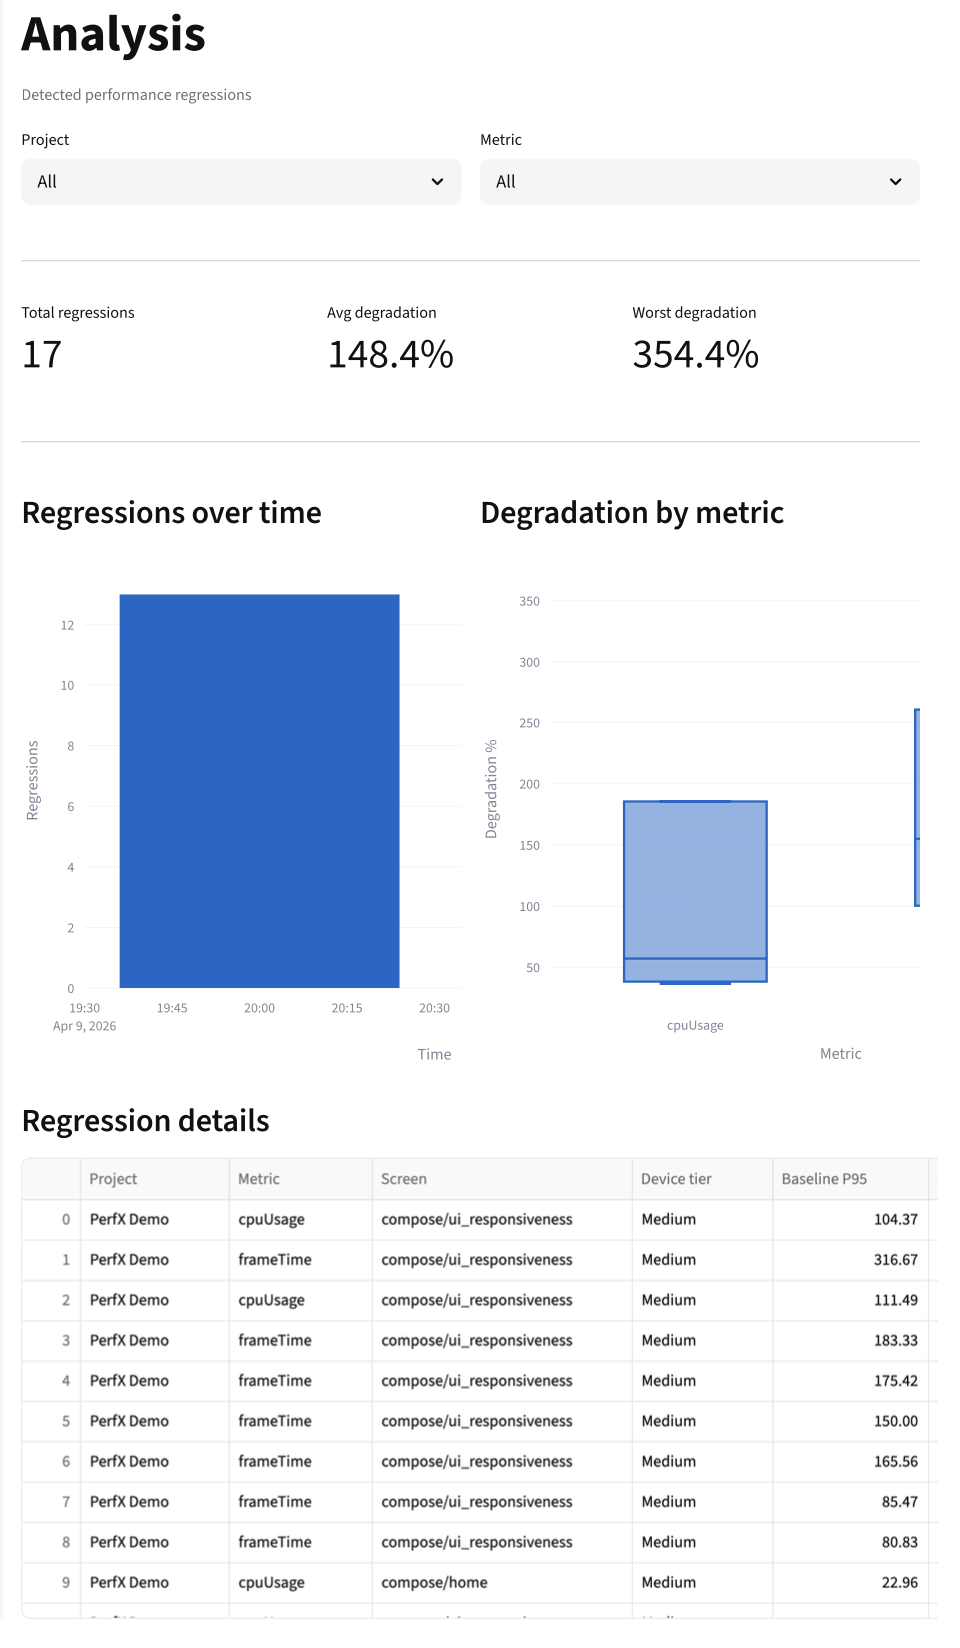
\includegraphics[width=0.8\textwidth]{figs/regression_analysis.png}
%     \caption{Regression analysis page}
%     \label{fig:frontend_metrics_2}
% \end{figure}

% \newpage 
\section{Performance Regression Detection Implementation}
\label{sec:regression_impl}

The regression detection pipeline described in Chapter~\ref{chap:met} was split into three stages: device cohort classification on the Ktor backend, data aggregation using ClickHouse queries, and statistical analysis using a Python service.

\subsection{Server-Side Cohort Classification}

The device cohort is calculated on the backend rather than on the mobile device. This decision was made so that the classification rules can be updated without requiring users to install a new version of the SDK. When the Ktor server receives a batch of metrics, it reads the hardware metadata (total RAM and CPU core count) from the request and assigns a cohort label before saving the record to ClickHouse.

\begin{lstlisting}[language=Kotlin, caption={Device cohort classification}]
fun calculateDeviceCohort(totalRamGb: Double, cpuCores: Int): String {
    return when {
        totalRamGb <= 3.0 -> "Low"
        totalRamGb <= 6.0 && cpuCores <= 8 -> "Medium"
        else -> "High"
    }
}
\end{lstlisting}

\subsection{ClickHouse Aggregation Queries}

To avoid loading large amounts of raw data into Python, the 95th percentile values for both the baseline and current windows are calculated directly in ClickHouse using the built-in \texttt{quantileIf} function. The query groups the results by metric type, screen name, and device cohort, which corresponds to the data partitioning described in Chapter~\ref{chap:met}.

\begin{lstlisting}[language=SQL, caption={ClickHouse query for P95 percentiles}]
SELECT
    metric_id, screen_name, device_cohort,
    quantileIf(0.95)(value, ts >= now() - INTERVAL 7 DAY
                            AND ts < now() - INTERVAL 1 DAY) AS baseline_p95,
    quantileIf(0.95)(value, ts >= now() - INTERVAL 1 DAY) AS current_p95
FROM metric_records
GROUP BY metric_id, screen_name, device_cohort
HAVING baseline_p95 > 0
\end{lstlisting}

\subsection{Statistical Validation}

After the percentiles are retrieved from the database, the Python service calculates the relative degradation for each combination of metric, screen, and device cohort. If the degradation exceeds the threshold configured by the developer (15\% by default), the system performs a Mann-Whitney U test on the raw data distributions to confirm that the change is statistically significant. The test is implemented using the \texttt{scipy.stats} library. If the resulting $p$-value is below 0.05, the regression is considered confirmed.

\begin{lstlisting}[language=Python, caption={Mann-Whitney U test for regression confirmation}]
from scipy.stats import mannwhitneyu

def validate_regression(baseline_data, current_data, threshold_delta):
    delta = (current_data.p95 - baseline_data.p95) / baseline_data.p95

    if delta > threshold_delta:
        stat, p_value = mannwhitneyu(current_data.raw_values,
                                     baseline_data.raw_values,
                                     alternative='greater')
        if p_value < 0.05:
            return True, p_value

    return False, None
\end{lstlisting}

\subsection{Automated Alerting}

When a regression is confirmed, the Python service saves it to the \texttt{regressions} table in PostgreSQL, recording the metric type, affected screen, device cohort, the calculated degradation percentage, and the $p$-value from the statistical test. After saving, the service sends a notification to the developer through the channel they configured in the dashboard (email or Telegram). The notification includes the name of the affected screen, the device cohort, the metric type, and the size of the degradation. Confirmed regressions are also displayed on the dashboard, where developers can filter and investigate active issues.

\section{Summary}

This chapter described the implementation of all four system components. The mobile SDK was built as a Kotlin Android library that collects six performance metrics using dedicated collectors, buffers the data in a two-tier storage layer, and transmits it to the backend in batches. The backend server uses Ktor to receive the data and stores it in two separate databases: ClickHouse for time-series metrics and PostgreSQL for user and project metadata. The frontend was built with Streamlit and provides dashboards, raw data exploration, and alert configuration. Finally, the regression detection pipeline was implemented as a Python service that runs ClickHouse aggregation queries and applies a statistical hypothesis test to confirm detected regressions. The next chapter evaluates how well this system works in practice.
